
\setchapterabstract{}
\chapter{Probability Theory}
\vspace{-1.5cm}

\setchapterabstract{
    This chapter introduces the fundamental concepts of probability theory. We begin by exploring the idea of experiments, outcomes, and sample spaces. Next, we define sigma algebras and discuss their properties. Finally, we introduce the concept of probabilities and how they are assigned to events, focusing on key properties such as additivity and independence. 
}
\chaptoc
\vspace{0.5cm}

\section{Experiments and Sample Spaces}

\begin{itemize}
    \item \(\Omega\) represents the set of all possible outcomes of an experiment. For example, if we roll a die, \(\Omega = \{1, 2, 3, 4, 5, 6\}\).
    \item \(\mathcal{A}\) is a collection of subsets of \(\Omega\) that satisfies:
        \begin{enumerate}
            \item \(\Omega \in \mathcal{A}\)
            \item If \(E \in \mathcal{A}\), then \(\bar{E} \in \mathcal{A}\)
            \item If \(E_1, E_2, \dots, E_n \in \mathcal{A}\), then \(\bigcup_{n=1}^\infty E_n \in \mathcal{A}\)
        \end{enumerate}
    \item Additional concepts:
        \begin{itemize}
            \item If \(E, F \in \mathcal{A}\), then \(E \cap F \in \mathcal{A}\)
        \end{itemize}
\end{itemize}

The simplest sigma algebra is \(\mathcal{A} = \{\Omega, \emptyset\}\).

\noindent The Power set of a finite set \(\Omega = \{a, b, c\}\):
\[
2^\Omega = \{\{a, b, c\}, \{a, b\}, \{b, c\}, \{a, c\}, \{a\}, \{b\}, \{c\}, \emptyset\}
\]
The power set contains \(2^{n}\) elements for a sample space with \(n\) elements.

\vspace{0.5cm}

\section{Probabilities}
A \textit{probability measure}, \(P\), is a function that assigns a real number to events in \(\mathcal{A}\). For each \(E \in \mathcal{A}\), we have \(P(E) \in [0, 1]\), and the following conditions hold:

\begin{itemize}
    \item \(P(\Omega) = 1\)
    \item Additivity: For disjoint events \(E_1, E_2, \dots\), 
    \[
    P\left( \bigcup_{n=1}^{\infty} E_n \right) = \sum_{n=1}^{\infty} P(E_n)
    \]
    \item For two events \(E\) and \(F\),
    \[
    P(E \cup F) = P(E) + P(F) - P(E \cap F)
    \]
\end{itemize}

\noindent Note, for three events:
\[
P(E \cup F \cup G) = P(E) + P(F) + P(G) - P(E \cap F) - P(E \cap G) - P(F \cap G) + P(E \cap F \cap G)
\]


\section{Combinatory}

\subsection{Permutations}
Permutations involve aligning \( n \) objects in \( n \) places. There are two key cases:
\begin{itemize}
    \item \textbf{Distinct objects (ex. mother):} All \( n \) objects are distinct, and we can arrange them in \( n! \) ways. For example, arranging 6 distinct objects in 6 places can be done in \( P_n = n! \) ways. Ex. Olympics possible arrivals.
    \[
    P_n = n! 
    \]
    \vspace{-0.5cm} % Reduce space between text and figure
    \begin{figure}[h]
        \centering
        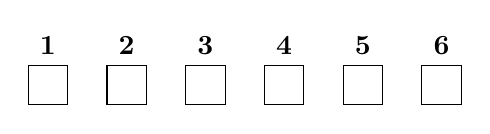
\begin{tikzpicture}
            % Six smaller boxes
            \foreach \i in {1,...,6} {
                \draw (\i, 0) rectangle (\i+0.5, 0.5); % Smaller boxes
                \node at (\i+0.25, 0.75) {\textbf{\i}};  % Numbers stay the same distance above
            }
        \end{tikzpicture}
        \caption{6 boxes for permutation}
    \end{figure}
    
    
    \item \textbf{Repetitive permutations (ex. mummy):} If some objects are repeated, we account for the repetition by dividing by the factorial of the count of the repeated objects. For example, arranging 5 objects where 3 are identical (mmm = 3 k1, u = 1k2, y = 1k3)can be done in:
    \[
    P_n = \frac{n!}{k_1! k_2! k_3! \dots} = \frac{5!}{3! 1! 1!}
    \]

\end{itemize}



\subsection{Dispositions}
Dispositions involve aligning objects in fewer places than the total number of objects. We consider two cases:
\begin{itemize}
    \item \textbf{Simple dispositions:} This involves choosing and aligning \( k \) objects from \( n \). For example, if we have 8 runners and we are selecting the top 3 positions, we compute:
    \[
    D_{n,k} = \frac{n!}{(n-k)!} = \frac{8!}{(8-3)!}
    \]
    \vspace{-0.5cm} % Reduce space between text and figure
    \begin{figure}[h]
        \centering
        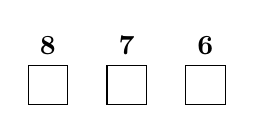
\begin{tikzpicture}
            % Three smaller boxes for simple dispositions
            \foreach \i in {1,...,3} {
                \draw (\i, 0) rectangle (\i+0.5, 0.5); % Smaller boxes
            }
            \node at (1.25, 0.75) {\textbf{8}};
            \node at (2.25, 0.75) {\textbf{7}};
            \node at (3.25, 0.75) {\textbf{6}};
        \end{tikzpicture}
        \caption{Simple dispositions}
    \end{figure}
    
    

    
    \item \textbf{With repetition:} When repetition is allowed, the number of dispositions is given by:
    \[
    D^*_{n,k} = n^k
    \]
    \vspace{-0.5cm} % Reduce space between text and figure
    \begin{figure}[h]
        \centering
        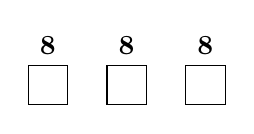
\begin{tikzpicture}
            % Three smaller boxes for repetition (all 8s)
            \foreach \i in {1,...,3} {
                \draw (\i, 0) rectangle (\i+0.5, 0.5); % Smaller boxes
                \node at (\i+0.25, 0.75) {\textbf{8}};  % Numbers stay the same distance above
            }
        \end{tikzpicture}
        \caption{Disposition with repetition}
    \end{figure}
    
    
\end{itemize}

\subsection{Combinations}
Combinations involve grouping objects, where the order does not matter. We calculate how many distinct subsets of k elements can be built out of n objects. For example, selecting 3 elements from a set can be done in:
\[
C_{n,k} = \frac{n!}{k!(n-k)!}
\]
Unlike permutations, combinations do not take into account the order of the elements. For example, a locker code is not a combination, but a permutation.  
Note the formula is just like the one for permutations but as here order does not matter we divide for the possible k positions that a single letter can take.

\section{Examples}

\Example{
    We are given a set of 6 green balls (G) and 4 red balls (R). If we pick 3 balls, we can explore the following cases:
    }


\textbf{Case 1: With repetition allowed} \\
We calculate the probability of drawing 3 green balls as:
\[
P(\text{3 greens}) = \frac{D^*_{6,3}}{D^*_{10,3}} = \frac{6^3}{10^3} = \frac{1}{6}
\]

\textbf{Case 2: Without repetition} \\
If we pick 3 balls without repetition, the probability is calculated as:
\[
P(\text{3 greens}) = \frac{D_{6,3}}{D_{10,3}} = \frac{6\cdot5\cdot4}{10\cdot9\cdot8} = \frac{1}{6}
\]

\textbf{Case 3: All the three balls extracted together} \\
In this case, we calculate the probability of drawing 3 green balls together:
\[
P(\text{3 greens together}) = \frac{C_{6,3}}{C_{10,3}} = \frac{1}{6}
\]
This is the same result as in Case 2, showing consistency across different experiment setups.


\Example{Example 2: Ten Balls, Each with a Number from 1 to 10, Extract Three Balls without Repetition}

\textbf{1. What is the probability that the third ball is even?}
A priori, we just know that the probability of drawing an even ball at each trial is \(\frac{1}{n}\).

\textbf{2. What is the probability that the numbers of the extracted balls are in increasing order (i.e., \(I < II < III\))?}
Ont of 10 elements, you can got 6 combinations for each 3 elements, of these 6, just one will be in increasing order \rightarrow out of 720 possible combinations, 120 will be in increasing order. Hence the potability will be \(\frac{120}{720}\)

\Example{In a group of \(n\) people, what is the probability that at least 2 people share the same birthday?}

1. \textbf{What is the probability that 2 persons share the same birthday?}

The complement of this event is the probability that no one shares the same birthday. We can use the formula for simple dispositions (without repetition) to find the number of ways to assign \(k\) distinct birthdays of \(k\) people out of the possibility of dispositions with repetitions:

\[
P(\overline{E}) =  \frac{D_{365, n}}{D^*_{365, n}}
\]
So, the probability that at least two people share the same birthday is:
\[
P(E) = 1 - P(\overline{E}) = 1 - \frac{365 \cdot 364 \cdot \dots \cdot (365 - n)}{365^n}
\]


2. \textbf{What is the probability that I share a birthday with one of these persons?}
Probability everyone is disposed with repetition in any other day then mine, over probability of disposition with repetition on any other day:
\[
P(\overline{E}) =  \frac{D^*_{365-1}}{D^*_{365}} \rightarrow P(E) = 1 - \left(\frac{364}{365}\right)^n
\]
As the number of people increases, the probability that at least one person shares a birthday with me increases as well.

\textbf{Example 4: Dimostrazione}

            \[ n \begin{cases}
                Letters \\
                Envelopes
            \end{cases} \]
        
            Let us assume there are two scenarios
        
            \[ \phi_1 = \text{probability that all the letters are in the right envelope} = \frac{1}{n!} \]
            \[ \phi_2 = \text{probability that no letter is in the right envelope} = \clubsuit \]
        
            We have two complementary probabilities, \(N\) and \(\Bar{N}\), described as:
        
            \[N = \Bar{E}_1 \cap \Bar{E}_2 \cap \ldots \cap \Bar{E}_n\]
            \[\Bar{N} = E_1 \cup E_2 \cup \ldots \cup E_n\]
        
            \begin{equation}
            \begin{split}
               & \mathbb{P} (N) = 1 - \mathbb{P} (\Bar{N}) = 1 - \mathbb{P} (E_1 \cup E_2 \cup \ldots \cup E_n) = \\ & 1 - \mathbb{P} (E_1) - \mathbb{P} (E_2) - \ldots - \mathbb{P} (E_n) + \mathbb{P} (E_1 \cap E_2) + \ldots + \mathbb{P} (E_{n-1} \cap E_n) - \ldots \\ & 
            \end{split}
            \end{equation}

            \begin{equation}
                1 - \left( \sum_{1 \leq i \leq n} \mathbb{P}(E_i) - \sum_{1 \leq i \leq j \leq n} \mathbb{P}(E_i \cap E_j) + \sum_{1 \leq i \leq j \leq k \leq n} \mathbb{P}(E_i \cap E_j \cap E_k) - \ldots + (-1)^n \mathbb{P} (E_1 \cap E_2 \cap E_3 \cap \ldots E_n)  \right)
            \end{equation}

            Note that:
            \[\mathbb{P} (E_i) = \frac{(n-1)!}{n!} = \frac{1}{n} \]
            \[\mathbb{P} (E_i \cap E_j) = \frac{(n-2)!}{n!} = \frac{1}{n(n-1)} \]
            \[\mathbb{P} (E_i \cap E_j \cap E_k) = \frac{(n-3)!}{n!} = \frac{1}{n(n-1)(n-2)} \]
            \[\mathbb{P} (E_1 \cap E_2 \cap E_3 \cap \ldots E_n) = \frac{0!}{n!} = 0 \]

            \begin{equation}
                1 - \left( n \cdot \frac{1}{n} - \binom{n}{2} \cdot \frac{1}{n(n-1)} + \binom{n}{3} \cdot \frac{1}{n(n-1)(n-2)} - \ldots + (-1)^n \cdot 0 \right)
            \end{equation}

            \begin{equation}
                1+ \sum_{k-1}^{n} (-1)^k \binom{n}{k} \frac{(n-k)!}{n!} = 1 + \sum_{k=1}^{n} (-1)^k \frac{1}{k!}
            \end{equation}

            \begin{equation}
                \mathbb{P} (N) = \sum_{k=0}^{n} (-1)^k \frac{1}{k!} \xrightarrow{n \to \infty} e^{-1}
            \end{equation}

            With 

            \[ e^{\alpha} = \sum_{k=0}^{\infty} \frac{\alpha^t}{k!} \]

\textbf{Example 5: Dimostrazione} 

            Given \(n\) keys, define \(E_j\) = "enters home at trial \(j\)"

                \begin{itemize}
                    \item \textbf{No key repetition}
                    
                        \begin{equation}
                            \mathbb{P} (E_j) = \frac{D_{n-1,j-1} \cdot D_{1,1} }{D_{n,j}} = \frac{(n-1)!}{n!} = \frac{1}{n} 
                        \end{equation}

                        This only holds true for \(j = 1,2, \ldots, n\), when the probability is \textit{a priori}.
                    
                    \item \textbf{With key repetition}
                    
                        \begin{equation}
                            \mathbb{P} (E_j) = \frac{D_{n-1,j-1}^* \cdot \overbrace{1}^{D_{1,j}}}{D^*_{n,j}} = \frac{(n-1)^{j-1}}{n^j} = \left( 1 - \frac{1}{n} \right)^{j-1} \cdot \frac{1}{n}
                        \end{equation}

                        Where the latter element of the equation is a series to 1.
                    
                \end{itemize}


\section{Independent Events}

        \subsubsection{Stochastic Independence}

            \Definition{
            Given the probability space \( ( \Omega, A, \mathbb{P} ) \), two events \(E, F \in A\) are said to be \textbf{stocastically independent} if \(\mathbb{P} (E) \cap \mathbb{P} (F) = \mathbb{P} (E) \cdot \mathbb{P} (F)\)
            \begin{equation}
                \mathbb{P} (E|F) = \mathbb{P} (E) \iff \mathbb{P} (F|E) = \mathbb{P} (F)
            \end{equation}
            }{Stochastic Independence}
            

        \subsubsection{Conditional Stochastic Independence}

            \Definition{
            Given the probability space \( ( \Omega, A, \mathbb{P} ) \) and the events \(A, B, F \), \textbf{Conditional Stochastic Independence} can be characterised as:
            \begin{equation}
                \mathbb{P} (A \cap B | F) = \mathbb{P} (A|F) \cdot \mathbb{P} (B|F)
            \end{equation}
            }{Conditional Stochastic Independence}

            \Warning{
            Stochastic Independence \textbf{does not imply} Conditional Stochastic Independence, and vice versa.
            }

            \section{Conditional Probability}
            
                In the probability space \( ( \Omega, A, \mathbb{P}) \), conditional probability can be written as
            
                \begin{equation}
                    \mathbb{P} (E|F) = \frac{\mathbb{P} (E \cap F)}{\mathbb{P} (F)}
                \end{equation}
            
                \noindent
                with \(\mathbb{P} (F) > 0\)
            
                
                    \subsubsection{Conditional Probability as Intersection of Events}
            
                        \begin{equation}
                        \begin{split}
                            \mathbb{P} (E \cap F) = & \mathbb{P} (F) \cdot \mathbb{P} (E | F) \\
                            \mathbb{P} (E_1 \cap E_2 \cap \cdots \cap E_n ) = & \mathbb{P} (E_1) \cdot \mathbb{P} (E_2 | E_1) \cdot \mathbb{P} (E_3 | E_2 \cap E_1) \cdots \mathbb{P} (E_n | E_1 \cap E_2 \cap \cdots \cap E_{n-1})
                        \end{split}
                        \end{equation}
            
                    \subsubsection{Law of Total Probability}
            
                        Given \(E_1, \ E_2, \ \cdots \ E_n\) partitions of \(\Omega\) and the conditions
            
                        \begin{enumerate}
                            \item \(E_i \cap E_j = \emptyset \forall i \neq j\)
                            \item \(E_1 \cup E_2 \cup \cdots \cup E_n = \Omega\)
                        \end{enumerate}
            
                        \noindent
                        We can state that:
            
                        \begin{equation}
                            \mathbb{P} (F) = \sum^{n}_{i=1} \mathbb{P} (F|Ei) \mathbb{P} (E_i)
                        \end{equation}
            
                    \subsubsection{Bayes Formula}
            
                        Given 
            
                        \begin{equation}
                            \mathbb{P} (E_n | F) = \frac{\mathbb{P} (F| E_n) \mathbb{P} (E_n)}{\sum^{n}_{i=1} \mathbb{P} (F|Ei) \mathbb{P} (E_i)} \rightarrow \mathbb{P} (A|P) \frac{\mathbb{P} (B|A) \mathbb{P} (A)}{\mathbb{P} (B)}
                        \end{equation}
            
            


            \textbf{Ex.1 Conditional Proabbility}

            \begin{table}[h!]
                \centering
                \begin{tabular}{|c|c|c|}
                    \hline
                    \textbf{Probability} & \textbf{Damaged} \\
                    \hline
                    \textbf{A}  & 0.5 & 0.06 \\
                    \hline
                    \textbf{B}  & 0.3 & 0.04 \\
                    \hline
                    \textbf{C}  & 0.2 & 0.08 \\
                    \hline
                \end{tabular}
                \caption{Example Table}
                \label{tab:example}
            \end{table}
            
            \begin{equation}
            \begin{split}
                \mathbb{P} (D) & = \mathbb{P} (D|A) \cdot \mathbb{P} (A) + \mathbb{P} (D|B) \cdot \mathbb{P} (B) + \mathbb{P} (D|C) \cdot \mathbb{P} (C) \\
                & = 0.06 \cdot 0.5 + 0.04 \cdot 0.3 + 0.08 \cdot 0.2 = 0.06 + 0.012 + 0.016 = 0.088
            \end{split}
            \end{equation}
            
            \begin{equation}
                \mathbb{P} (B|D) = \frac{\mathbb{P}(D|B) \mathbb{P}(B) }{\mathbb{P}(D)} = \frac{\mathbb{P} (B \cap D)}{\mathbb{P} (D)} = \frac{0.04 \cdot 0.3}{0.088} = \frac{0.012}{0.088} = 0.136
            \end{equation}
            
            \textbf{Ex.2 Conditional Probability}
            
            \[\mathbb{P} (t_+ | ill) = 0.98 \]
            \[\mathbb{P} (t_- | not \ ill) = 0.99 \]               
            
            Given \( \mathbb{P}(ill) = p  \)
            
            \begin{equation}
                \rightarrow \mathbb{P} (ill | t_+) = \frac{\mathbb{P} (t_+ | ill)\mathbb{P} (ill)}{\mathbb{P}(t_+)} = \frac{0.98 \cdot p}{\mathbb{P}(t_+)} = \frac{0.98 \cdot p}{0.98 \cdot p + 0.01 \cdot (1-p)} 
            \end{equation}
            
            \textbf{Ex.3 Conditional Probability}
            
            Image we toss two dices
            
            \[ \Omega = \left\{ (1,1),(1,2),(1,3) \ldots \right\} \]
            
            What's \( \mathbb{P} (E) \), given \(E\) : "sum is 8" and that \(F\) = first toss = 5?
            
            \begin{equation}
            \begin{split}
                \mathbb{P} (E|F) & = \frac{1}{6} \\
                \mathbb{P} (E) & = \frac{5}{36} \\
            \end{split}
            \end{equation}
            
            Two events $E$ and $F$ are positively correlated wgenever $\mathbb{P} (E|F) > \mathbb{P} (E)$ $\rightarrow$ $\mathbb{P} (E \cap F) > \mathbb{P} (E) \cdot \mathbb{P} (F)$
            
            

\section{Random Variables}

        Given the sample space of tossing a dice \(\Omega = \{1,2,3,4,5,6\} \), we can define:

            \[X: \Omega \rightarrow \mathbb{R} \]

        \Remark{
        In the equation above:
                \begin{itemize}
                    \item if \(\Omega\) is finite \(\rightarrow\) it is a random variable
                    \item if \(\Omega\) is discrete \(\rightarrow\) it is \textbf{not} a random variable 
                \end{itemize}
        }

        \noindent
        Properties to be considered a random variable:

            \begin{itemize}
                \item \(\forall t \in \mathbb{R}\)

                    \( \{ \omega \in \Omega : X (\omega) \leq t \} = E_t \in A \)

                    With \(X\) being \textbf{Borel measurable}

                \item 

                    \( \mathbb{P} (E_t) = \mathbb{P} (\omega \in \Omega : X (\omega) \leq t ) = \mathbb{P} (X (\omega) \leq t) = \mathbb{P} (X \leq t)  0 F_x (t)  \)
 
                \item \(F_x : \mathbb{R} \rightarrow \mathbb{R}\), with \(F_x(t)\) being the distribution function of the variable.

                    \( \lim _{t \to - \infty} F(t) = 0 \)    

                    \( \lim _{t\to\infty} F(t) = 1\)

                    \begin{itemize}
                        \item If \(X\) is discrete, the graph will possess the following properties:
                            \begin{enumerate}
                                \item Stepwise
                                \item Non-decreasing 
                                \item \(F_x\) continuous from the right
                            \end{enumerate}
                        \item If \(X\) is \textcolor{dblue}{absolutely} continuous
                            \begin{enumerate}
                                \item \(F\) is continuous
                            \end{enumerate}
                    \end{itemize}
            \end{itemize}

            \begin{figure}[h]
                \centering
                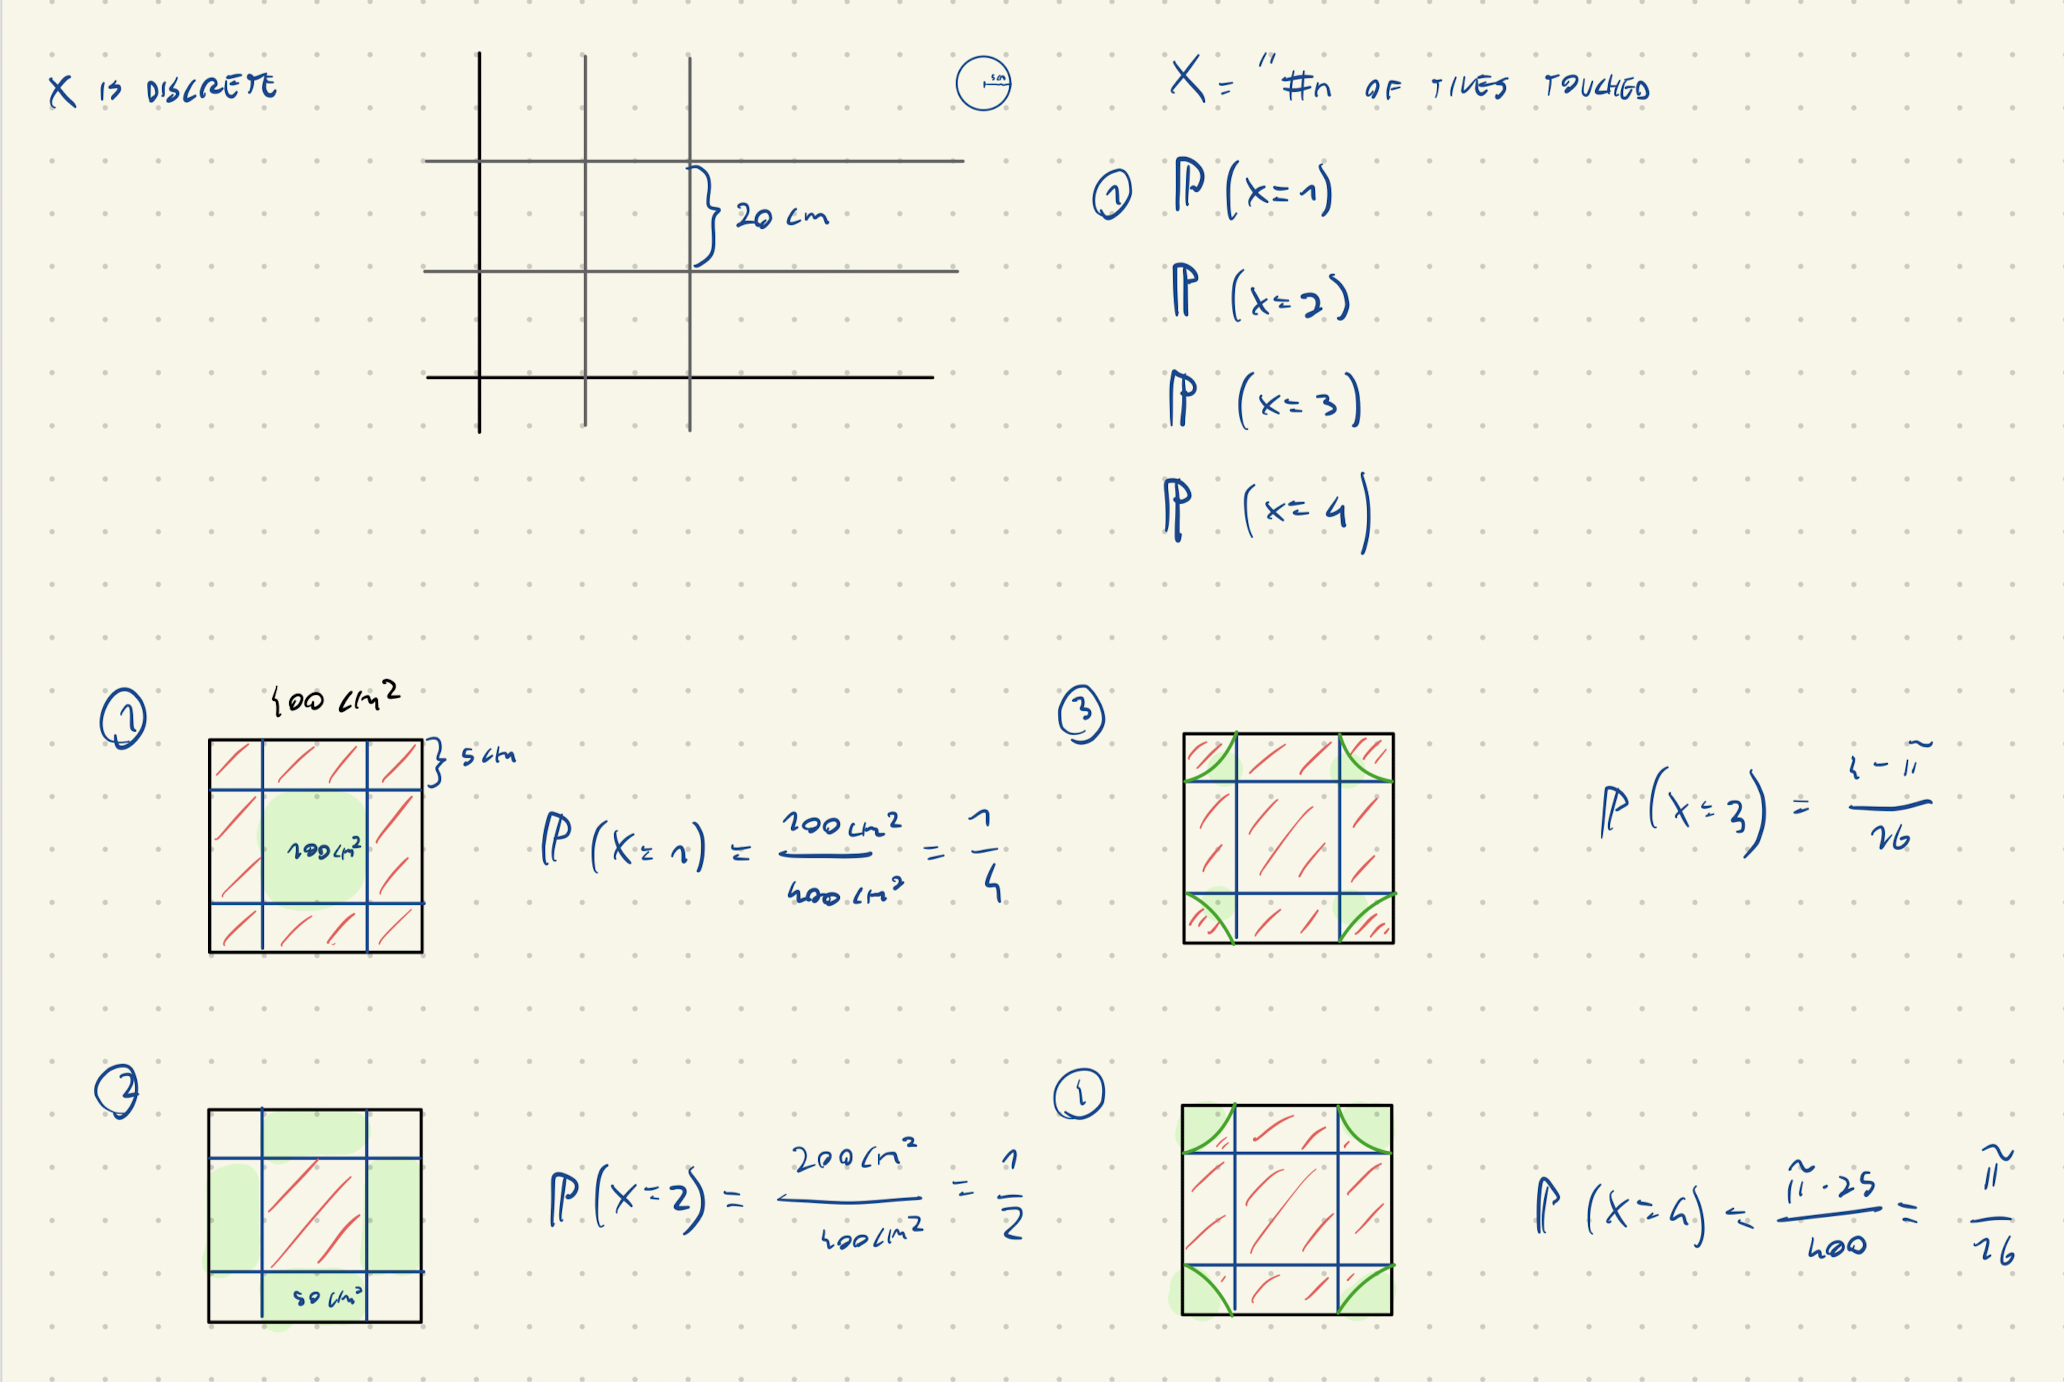
\includegraphics[width=0.90\linewidth]{X_visual_discrete.png}
                \caption{Visual representation of an example where \(X\) is a \textbf{discrete} random variable}
                \label{fig:X_visual_discrete}
            \end{figure}

            \begin{figure}[h]
                \centering
                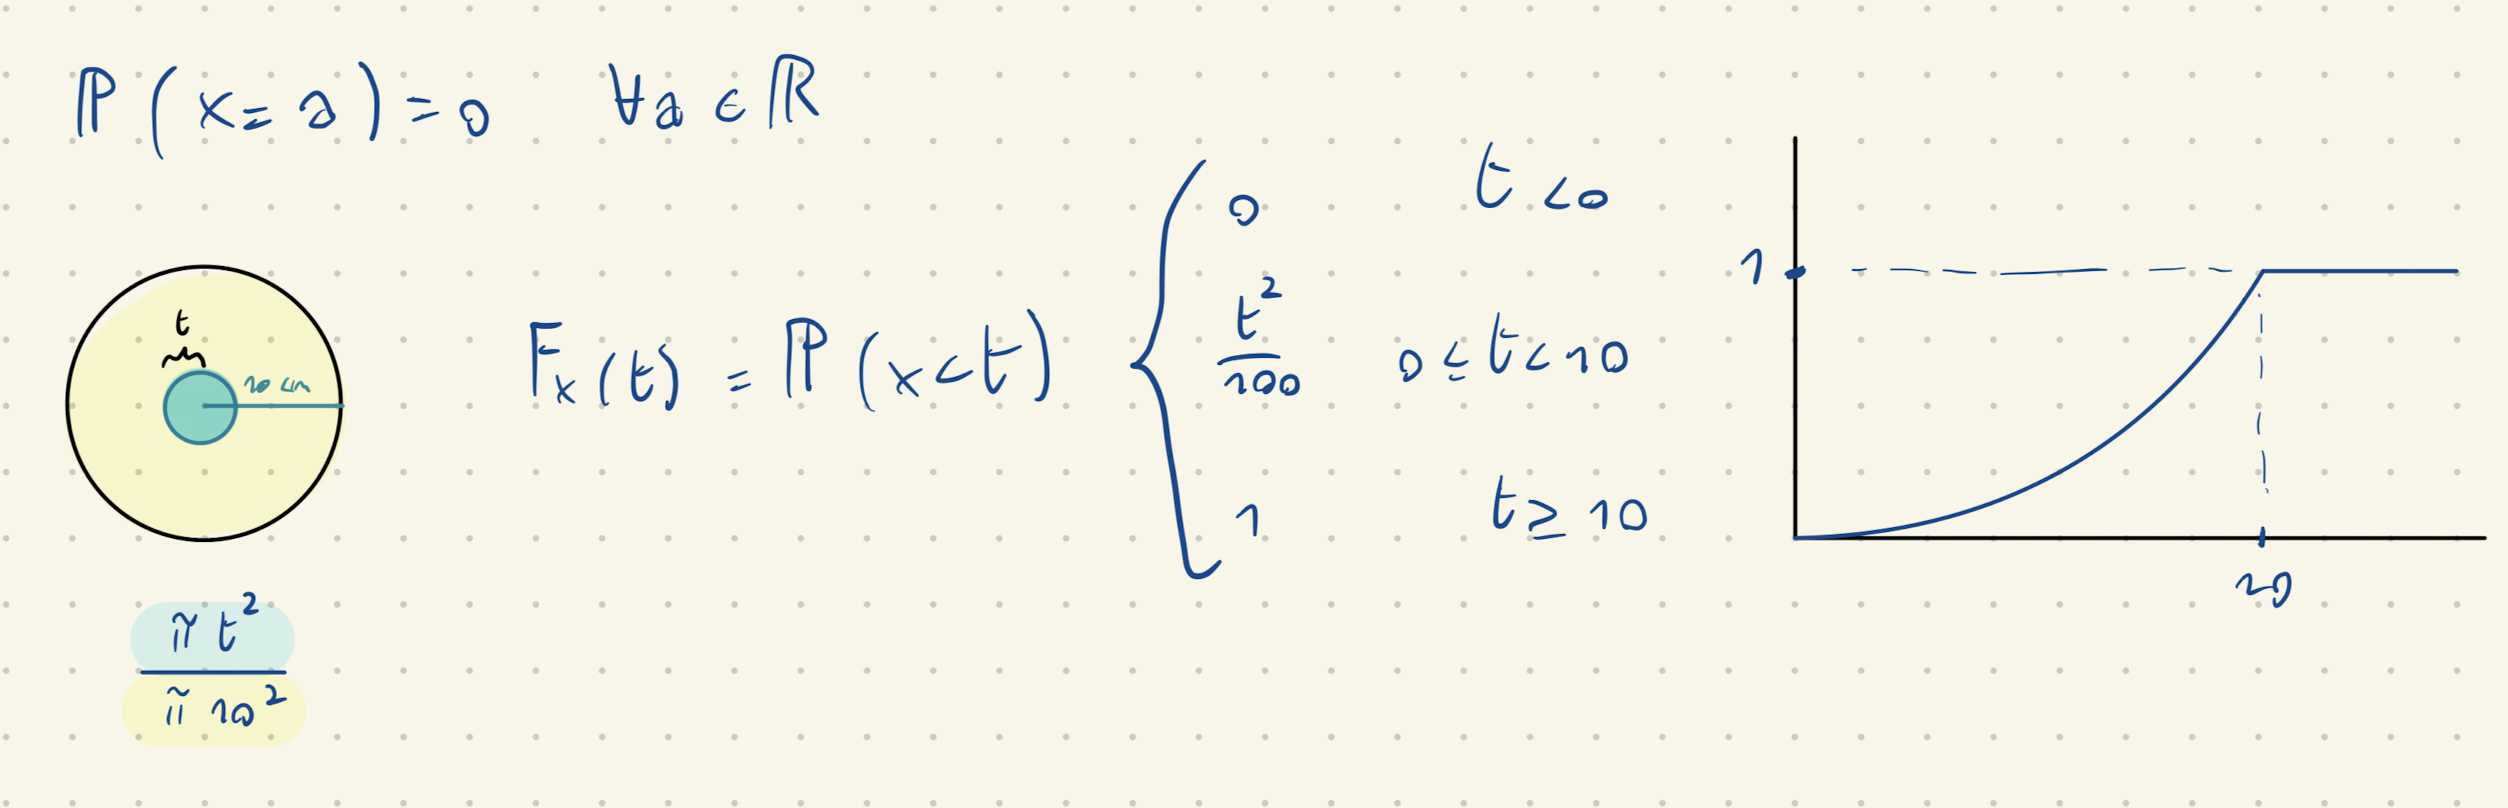
\includegraphics[width=0.90\linewidth]{X_visual_absolutely_continuous.png}
                \caption{Visual representation of an example where \(X\) is an \textbf{absolutely continuous} random variable}
                \label{fig:X_visual_absolutely_continuous}
            \end{figure}

            